{
\usebackgroundtemplate{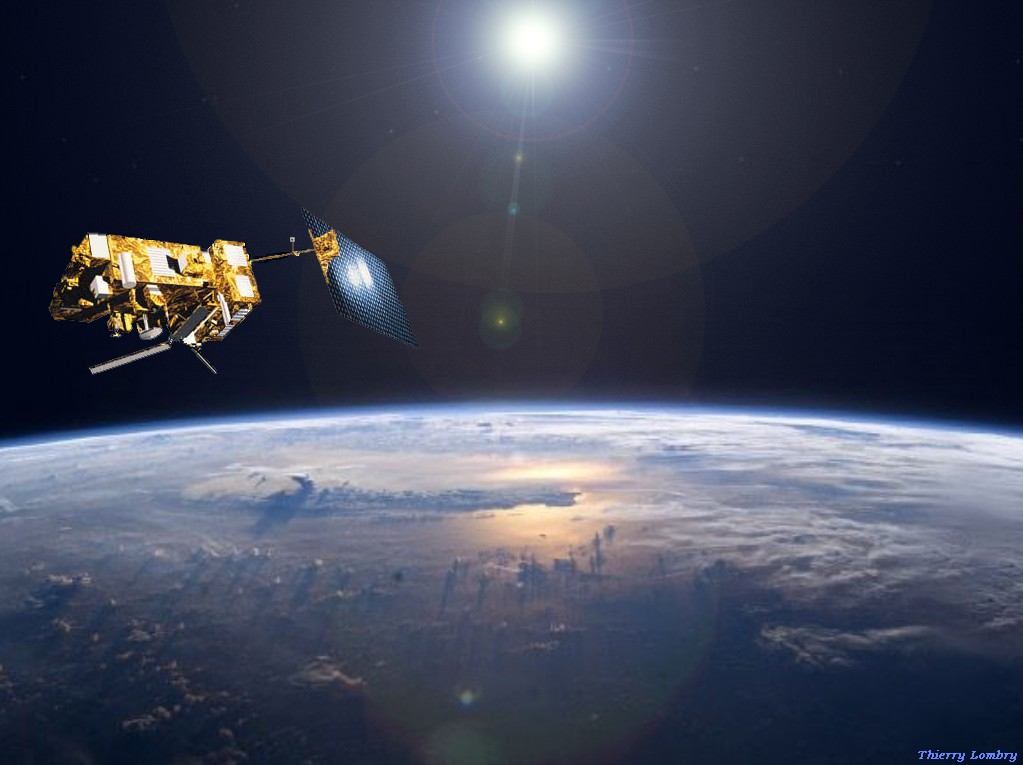
\includegraphics[height=\paperheight, keepaspectratio]{images/low_orbit}}%
\begin{frame}
\end{frame}
\begin{frame}
    \frametitle{About that circularizing}
    \begin{block}{}
        We are now almost in low earth orbit but still falling down. Our orbit could still cross the atmosphere.
        So we need to learn how to manipulate our orbit while in space.
    \end{block}
    \begin{block}{Basics}
        Movement on an orbit generally affects the opposite side of the orbit.
    \end{block}
\end{frame}
\begin{frame}
    \frametitle{Adjusting orbits}
    \begin{block}{}
        \begin{center}
            At any point on the orbit you can burn in 3 directions: up/down, left/right, forwards/backwards
        \end{center}
    \end{block}
    \begin{block}{}
        \begin{center}
            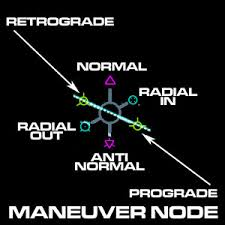
\includegraphics[scale=0.8]{images/maneuver_node}
        \end{center}
    \end{block}
\end{frame}
}

\begin{frame}
    \frametitle{Prograde}
    \begin{block}{}
        Burning in the prograde direction expands the size of the orbit, with the center of expansion at the current
        position.
    \end{block}
    \begin{center}
        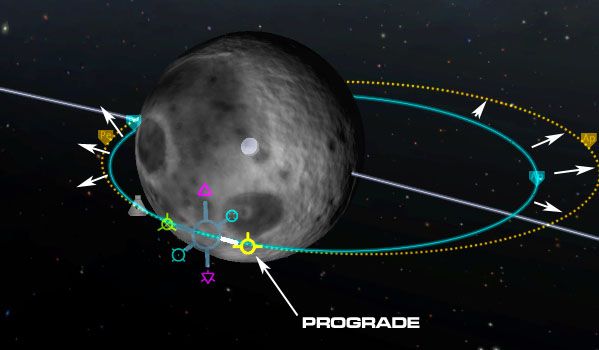
\includegraphics[scale=0.4]{images/prograde}
    \end{center}
\end{frame}
\begin{frame}
    \frametitle{Retrograde}
    \begin{block}{}
        Burning in the retrograde direction contracts the size of the orbit, with the center of contraction at the
        current position.
    \end{block}
    \begin{center}
        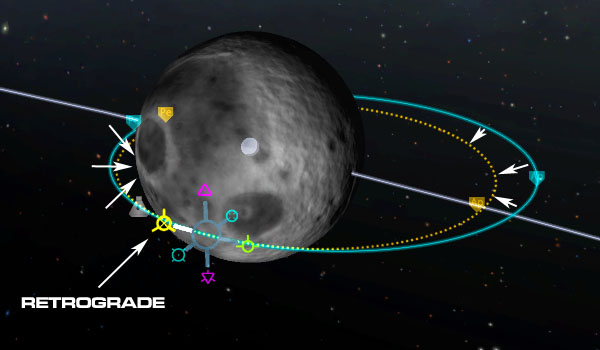
\includegraphics[scale=0.5]{images/retrograde}
    \end{center}
\end{frame}
\begin{frame}
    \frametitle{Normal}
    \begin{block}{}
        Burning in the normal direction tilts the orbital plane counterclockwise on the axis determined by the current
        position and the planet's center.
    \end{block}
    \begin{center}
        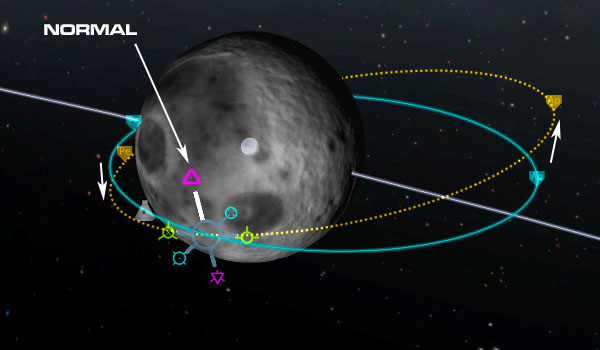
\includegraphics[scale=0.5]{images/normal}
    \end{center}
\end{frame}
\begin{frame}
    \frametitle{Anti-normal}
    \begin{block}{}
        Burning in the anti-normal direction tilts the orbital plane clockwise on the axis determined by the current
        position and the planet's center.
    \end{block}
    \begin{center}
        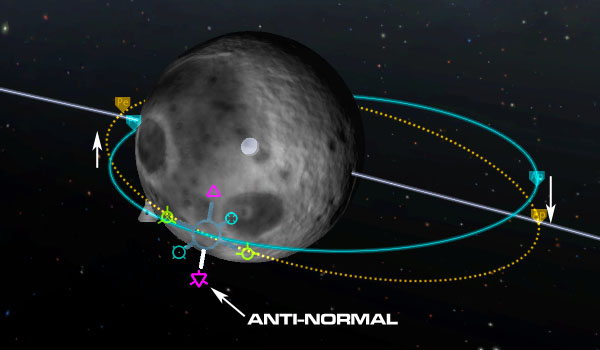
\includegraphics[scale=0.4]{images/anti_normal}
    \end{center}
\end{frame}
\begin{frame}
    \frametitle{Radial in}
    \begin{block}{}
        Burning in the radial-in direction rotates the orbial plane counterclockwise.
    \end{block}
    \begin{center}
        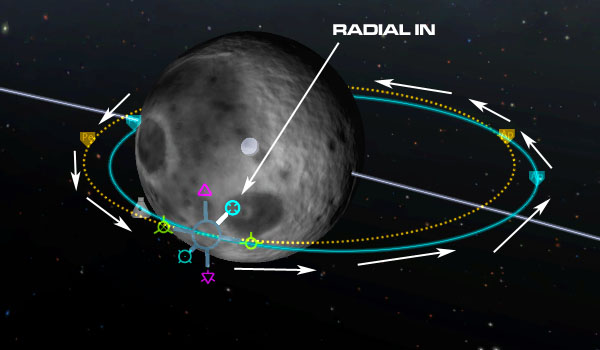
\includegraphics[scale=0.5]{images/radial_in}
    \end{center}
\end{frame}
\begin{frame}
    \frametitle{Radial out}
    \begin{block}{}
        Burning in the radial-out direction rotates the orbial plane clockwise.
    \end{block}
    \begin{center}
        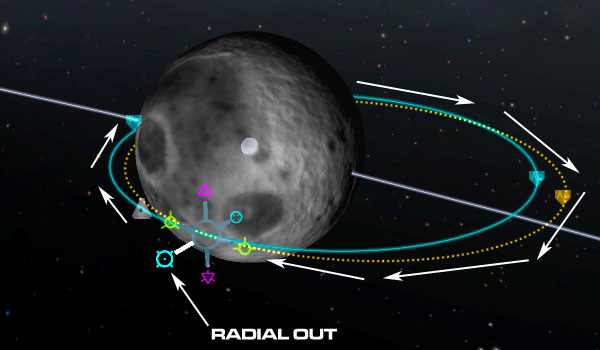
\includegraphics[scale=0.5]{images/radial_out}
    \end{center}
\end{frame}
